\chapter{Sprint 2}
\label{chap:S2}
In the second sprint, and our fourth week, of the project the first draft of a product backlog was created. The main focus of the sprint was on dividing work efforts both into working with the system development as well as on writing the report. As every other sprint, the group had the goal to be able to display a demo for the customer at the end of the sprint. In addition, toward the end of the sprint there was a presentation in Oslo, where the group was given the opportunity to show a working product to end users and receive feedback.

\section{Sprint Plan}
\label{sec:S2Plan}
As the first draft of a product backlog had now been created, the group was able to pull a number of items off the product backlog and into the sprint backlog, as shown in tables \ref{tab:S2BacklogP1} and \ref{tab:S2BacklogP2}. As most members were inexperienced in the field of web application development, and had used the previous sprint getting to know the technology better, this was the first Sprint where inexperienced started contributing to the implementation. 

\paragraph{}For cooperative programming simultaneously without causing inconsistency in the project files, the group was introduced to Git and GitHub by the members with previous experience with the technology.

%%%%%%%%%%%%
%Template for Figures %
%%%%%%%%%%%%
\begin{figure}[ht!]
\centering

\includegraphics[width=90mm]{Sprint2/img/Sprint2-GitnGithub.png}
\caption{Git and GitHub \label{fig:S2PlanGit}}
\end{figure}

\paragraph{} From the beginning of the system development the back and front end development have been closely connected. For this reason, it was necessary to make sure every member was aware of how to structure the project files concerning the website. As the technical lead, Valerij, briefly went through how a website is usually structured and how we would adapt this structure to our own project.

\paragraph{} At this stage, coding was separated into branches. Everyone working on the implementation tested their own code, with the help of others when necessary. Throughout this project, merging branches into the master branch on GitHub required that the code in that branch is fully functional. When merged into the master branch integration testing was done to make sure that the merge went smoothly and that the code of the master branch ran without errors.

\section{Duration and Workload:}
\label{sec:S2Duration}
%%%%%%%%%%%%%%%%
%Template for Sprint Duration %
%%%%%%%%%%%%%%%%
\begin{minipage}{\linewidth}
\centering
\setlength{\tabcolsep}{22pt}
\textbf{Sprint 2:} 
\smallskip
\rowcolors{1}{blue!20}{blue!10}
\begin{tabular}{ |l l| }
	\hline
	\it{Duration} & 2 weeks \\
	\it{Start} & September 22nd. \\
	\it{End} & October 5th. \\
	\it{Workload} & Hours spent by the entire group on Sprint 2. \\
	\it{Goal} & 40 - 50 hours per person \\
	\hline
\end{tabular}
\end{minipage}
%
\bigskip
%
%%%%%%%%%%%%%%%%
%Template for Sprint Workload %
%%%%%%%%%%%%%%%%
\begin{minipage}{\linewidth}
\setlength{\tabcolsep}{25pt}
\centering
\rowcolors{1}{blue!20}{blue!10}
\begin{tabular}{ |l|l| }
	\hline
	\multicolumn{2}{|c|}{\cellcolor{gray!25} Workload} \\
	\hline
	\it{Planning} & 85 hrs\\
	\it{Development} & 97 hrs \\
	\it{Design} & 17 hrs \\
	\it{Documentation} & 22 hrs \\
	\it{Testing} & 15 hrs \\
	\it{Learning} & 21 hrs \\
	\hline
	\it{Total workload} & 257 hrs \\
	\hline
\end{tabular}
%Caption here
\captionof{table}{Workload of Sprint 2.} 
\end{minipage}

\bigskip 

\paragraph{} This sprint the group managed to work 18.4 hours per person per week. This is only a very slight improvement from the previous sprint. This is a good sign, as we are moving in the right direction, but there is still room for improvement. This is discussed further in section \ref{sec:S2Retrospective}.

\section{Product Backlog}
\label{sec:S2Backlog}
Below is the first version of the product backlog. As we were aware of the major functions required for the project, and had come quite far on developing the system requirement document, the first version of our product backlog was of some use to assign items to the Sprint 2 backlog. Unfortunately, it did not take long before we realized that this first version did not scale very well with the rapidly increasing size of the backlog. 

%%%%%%%%Figure%%%%%%%%%
\begin{figure}[ht!]
\centering
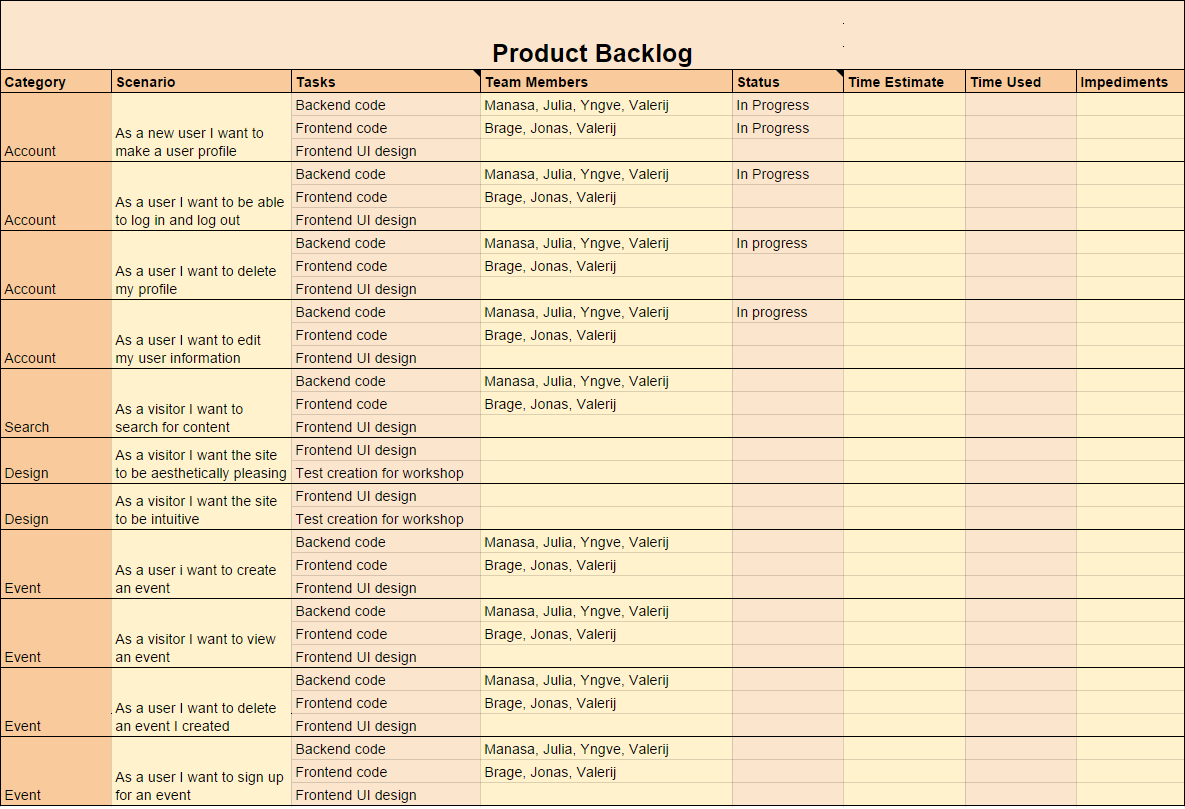
\includegraphics[width={\linewidth}]{Sprint2/img/Sprint2-FirstProductBacklog.png}
\caption{First Product Backlog. \label{fig:S2BacklogFirst}}
\end{figure}

\section{Sprint Backlog}

Below is a table of the backlog for the second sprint. \\ D: Design, F:Feature, TA: Task, TE: Test, 

%%%%%%%%%%%%%%%%%%%
%Template for Sprint Backlog table    %
%%%%%%%%%%%%%%%%%%%
\begin{minipage}{\linewidth}
\setlength{\tabcolsep}{12pt}
\centering
\rowcolors{1}{blue!20}{blue!10}
\begin{tabular}{|p{1cm}|p{4cm}|p{2cm}|p{2cm}|}
\hline
\cellcolor{gray!25} ID & \cellcolor{gray!25} Description & \cellcolor{gray!25} Estimated Time & \cellcolor{gray!25} Actual Time \\
\hline
TA2.1 & \it{Structurize Google Drive folders, and use the same language in all documents.} & 1 week & 21h \\
TA2.2 & \it{Set up NTNU home area for running and testing code.} & 2h & 2h \\
TE2.3 & \it{Use NTNU's MySQL server over SSH for testing database of user sign up, user creation, validation etc. } & 4h & 4h \\
D2.4.1 & \it{Find and apply a theme color for the web page. } & 3h & 4h \\
D2.4.2 & \it{Find and apply a background color for the web page.} & 3h & 4h \\
D2.5.1 & \it{Registration form: Layout.} & 1h & 3h \\
F2.5.1 & \it{Registration form: Sign up back end.} & 1w & 20h \\
D2.6.1 & \it{Sign in form: Layout.} & 1h & 1h \\
F2.6.1 & \it{Create the sign in form.} & 2h & 2h \\
F2.6.2 & \it{Validation used to make sure that all input fields are valid before saving to the database. } & 2h & 2h\\
\hline
\end{tabular}
\captionof{table}{Backlog Sprint 2, part 1. \label{tab:S2BacklogP1}} 
\end{minipage}

\begin{minipage}{\linewidth}
\setlength{\tabcolsep}{12pt}
\centering
\rowcolors{1}{blue!20}{blue!10}
\begin{tabular}{|p{1cm}|p{4cm}|p{2cm}|p{2cm}|}
\hline
\cellcolor{gray!25} ID & \cellcolor{gray!25} Description & \cellcolor{gray!25} Estimated Time & \cellcolor{gray!25} Actual Time \\
\hline
D2.7.1 & \it{Logo icon and logo text.} & 1h & 1h \\
D2.7.2 & \it{Sign in button and Sign out button.} & 1h & 1h \\
D2.7.3 & \it{Sign up button.} & 1h & 1h \\
D2.7.4 & \it{Validation of forms: Error message with styles when invalid information is input.} & 1h & 1h \\
F2.7.1 & \it{Back-end functionality of sign in and sign out.} & 2h & 3h \\
F2.7.2 & \it{Back-end functionality for sign up and user creation.} & 2h & 3h \\
F2.7.3 & \it{Back-end functionality for validation check of forms.} & 2h & 3h \\
D2.8.1 & \it{Center photo posts, taking the map-sidebar-search into account.} & 1h & 1h \\
F2.8.3 & \it{Commenting on photos} & 6h & 7h \\
F2.8.2 & \it{Mouse-hover on photos enlarge.} & 1h & 2h \\
R2.9.1 & \it{Update and finish the Requirements Specification Document.} & 4h & 5h \\
\hline
\end{tabular}
\captionof{table}{Backlog for Sprint 2, part 2. \label{tab:S2BacklogP2}} 
\end{minipage}

\section{Presentation in Oslo}
\label{sec:S2Presentation}

As mentioned in chapter \ref{chap:Planning}, the customer had informed us early on in the project that there would be a workshop in oslo to present the ideas and possibly show off a demo of the final product. At the customer meeting on the 29th of September, the date for this workshop was confirmed to the 2nd of October. The workshop had been replaced with a presentation, but this would still give us the opportunity to gather some feedback from the target audience. The customer expected us to bring what we had and hold a presentation showcasing our plans for the product, with regards to both design and functionality. Because of this, the second week of this sprint focused on preparing the product for showcasing in Oslo.

\subsection{Preparation for the Presentation}
\label{subsec:S2PresentationPreparation}
The group decided that only two people would go to Oslo, as the rest of the team had other assignments and work, and did not have the time to travel. Work on the report was postponed to the next sprint to make sure our implementation was as good as possible. The group decided to have these functionalities ready for the presentation:

\begin{itemize}
  \item When clicking on an image it should show up as an overlay, with the possibility for commends under it.
  \item Creating an event.
  \item Create event button.
  \item Create event page.
\end{itemize} 

The back-end for these were not all completed. The create event part was sparse, and only some of the front end for it was complete before the presentation.

\paragraph{} We were also very interested in the current usability of our site, and beyond any open feedback, we also had some questions for the youth.

\begin{itemize}
  \item Do you have any comments regarding the design of the site to facilitate finding other people with the same interests as you.
  \item What do you think about the color scheme and design in general.
  \item Map
  \begin{itemize}
    \item Can you find areas on the map?
    \item Can you find your home on the map?
    \item Other comments regarding the map
  \end{itemize}
  \item Registration form
  \begin{itemize}
    \item Personal details.
    \item User anonymity: User name, full name, or first name?
  \end{itemize}
\end{itemize}

\subsection{Feedback}
\label{subsec:S2PresentationFeedback}

We got lots of feedback from end users, some very good and some of it less so.  In chapters \ref{chap:S4} and \ref{chap:S5}, we will discuss the features that made it into the scope of our project, while chapter \ref{chap:Further} will discuss features we consider important, but beyond the scope of this project. The complete feedback is listed here in a rough order of importance:

\begin{enumerate}
  \item Should have a mobile app that integrates the phone's camera to enable one-click upload.
  \item The search map is too small. Events should be displayed in the map as well as in the feed when selected.
  \item You should be able to search for places and addresses in the map, as well as filter by interests.
  \item Pictures (and other media) should display some information when selected, like interests, location and maybe the uploader.
  \item Consider following as a possibility (the kids really wanted this feature) 
\end{enumerate}

Some more feedback that is more difficult to place in order of importance.

\begin{itemize}
  \item When someone comments on content you uploaded you should be notified in some way.
  \item Consider some way of connecting this to Facebook (sharing photos).
  \item Enable support for some kind of direct user to user messaging.
  \item Some form of reward for use, like meeting new friends and getting feedback when people interact with your content (Like button/user rating).
  \item Connect an email to your account, and display this in place of username.
  \item Returning to the idea of a digital scene - positive responses.
  \item When registering as a new user you should be automatically logged in.
  \item Anonymity: depends on context, event organizers should have some contact information available, especially for larger arrangements
  \item Tips on how to create exposure. This will be discussed in chapter \ref{chap:Further}.
  \item Some way to invite some other users or notify them of an activity in order to not be completely alone if no one comes.
  \item Enable simultaneous upload of content to AS and FB Instagram and Youtube etc.
\end{itemize}


\section{Design and Implementation} 
\label{sec:S2DesignImpl}
The design and implementation phase of the second sprint includes several changes in design and implementation focusing on the features regarding signing up, logging in and logging out. 

\subsection{Design}
\label{subsec:S2DesignImplDesign}
%\textbf{Design} \\ 
The design of the sprint includes updates in color, creation of different forms, the header, and on the photo search page. The theme color of the website was set to a hard orange. Buttons, logo, borders, forms, etc. all inherit the theme color. The background color was set to gray, with a hint of orange. Further designs update the creation of a navigation bar, as a part of the header. The navigation bar includes the logo and icon, also designed in this phase. \\%
%
%%%%%%%Picture of Sprint Logo and Icon%%%%%%%
\begin{figure}[ht!]
\centering

\includegraphics[width=50mm]{Sprint2/img/Sprint2-logo1.png}
\caption{First icon and logo of the page in orange. \label{overflow}}
\end{figure}

\paragraph{} Buttons for signing up, signing in, signing out, and creating an event, were created during this phase for the navigation bar. All buttons are clickable and animated to show a button push. \\%
%
%%%%%%%%%Pictures of buttons. %%%%%%%%%%%%
\begin{figure}[ht!]
\centering

\includegraphics[width=40mm]{Sprint2/img/Sprint2-buttons1.png}
\caption{Navigation buttons before signing in. \label{overflow}}
\end{figure}

%%%%%%%%%%% Button2 %%%%%%%%%%%
\begin{figure}[ht!]
\centering

\includegraphics[width=40mm]{Sprint2/img/Sprint2-buttons2.png}
\caption{Navigation buttons after signing in. \label{overflow}}
\end{figure}

\paragraph{}
Next was the design of the sign in form and the sign up form. These are simple forms, that pop up in an overlay window when the corresponding buttons are pushed in the navigation bar. \\

%%%%%%%%%% Figure: Sign in %%%%%%%%%%%%
\begin{figure}[ht!]
\centering
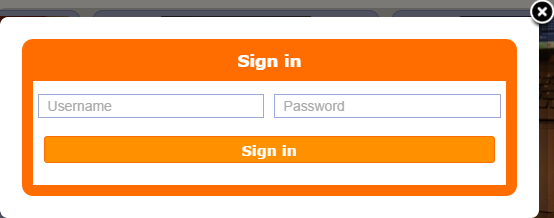
\includegraphics[width=90mm]{Sprint2/img/Sprint2-SignInForm.png}
\caption{The sign In form. \label{overflow}}
\end{figure}

%%%%%%%%%%%%% Figure sign up %%%%%%%%%%%
\begin{figure}[ht!]
\centering
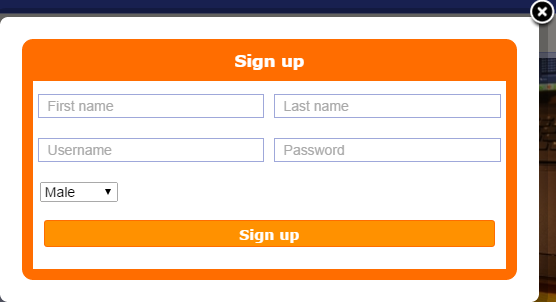
\includegraphics[width=90mm]{Sprint2/img/Sprint2-SignUpForm.png}
\caption{The sign Up form. \label{overflow}}
\end{figure}

\paragraph{} For the media search page, the media posts were updated to be correctly centered and also enlarged upon mouse hover. See below. 

%%%%%%%%%% Figure: Photo page %%%%%%%%%%
\begin{figure}[ht!]
\centering
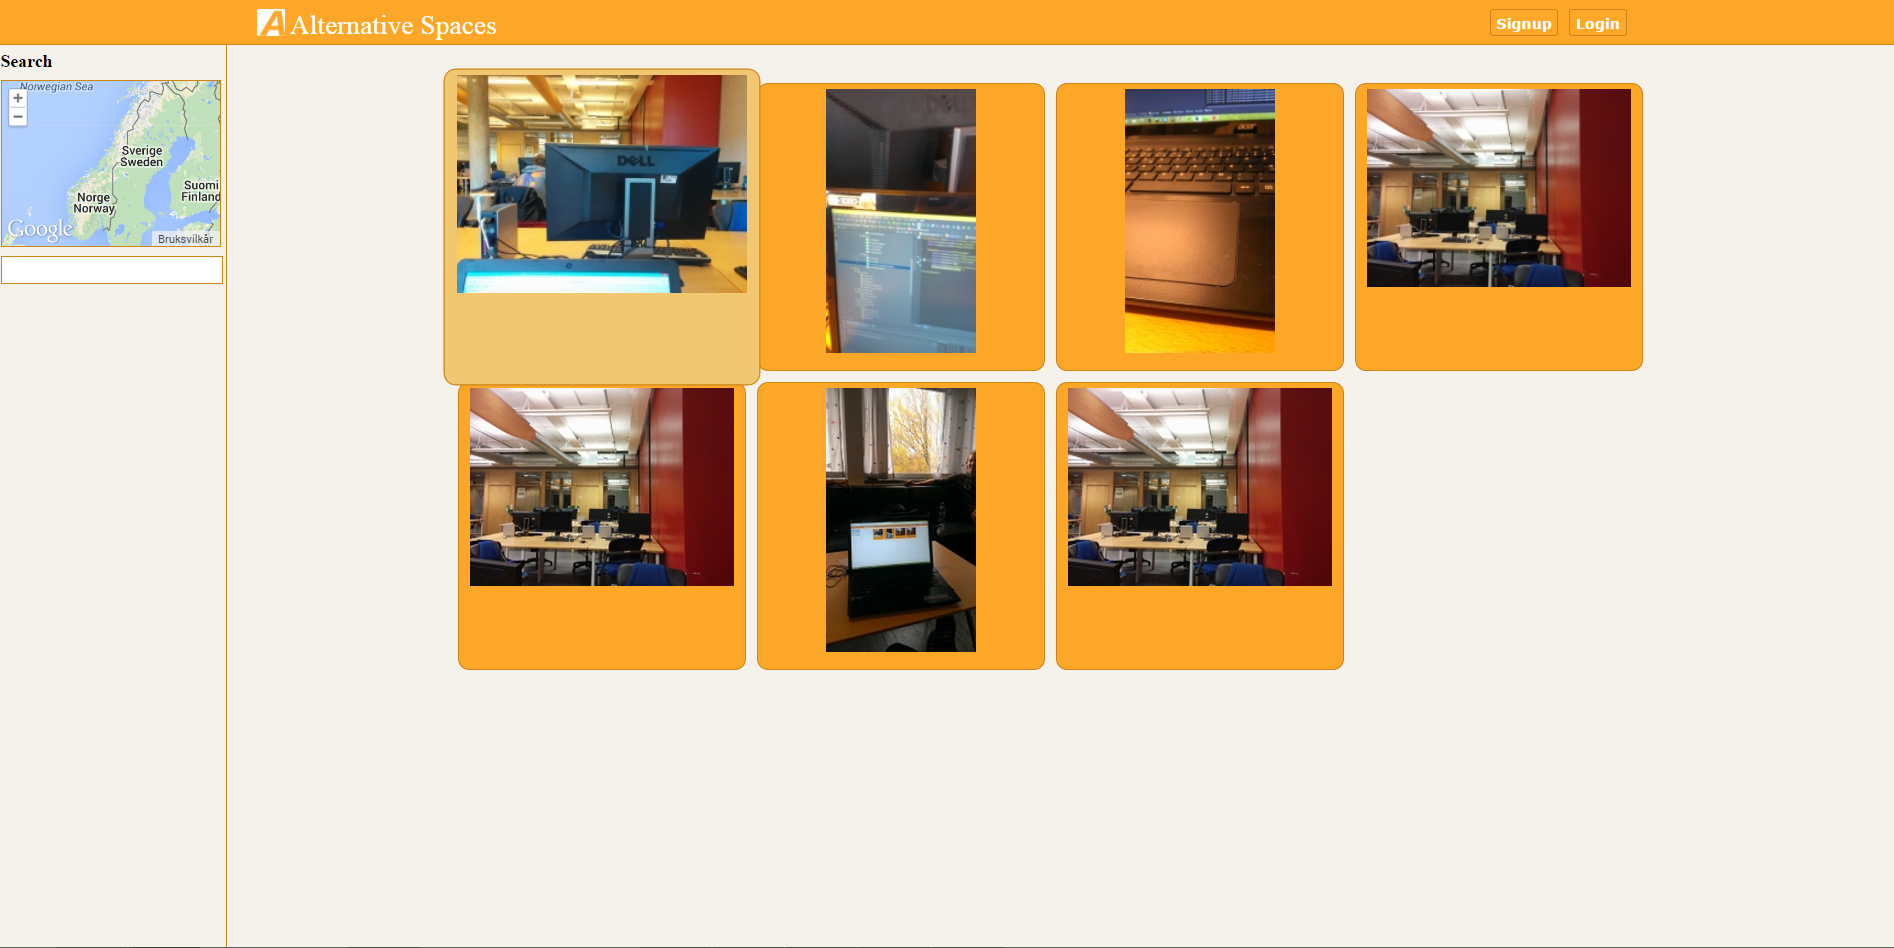
\includegraphics[width={\linewidth}]{Sprint2/img/Sprint2-PhotoPage.png}
\caption{The photo and location search page, with correctly centered media with the first post enlarged on hover. At the top is the full navigation bar, and on the left side is the map sidebar. \label{overflow}}
\end{figure}


\subsection{Implementation}
\label{subsec:S2DesignImplImpl}
For the implementation phase of the second sprint, on the back-end, most work complements what was discussed in the design section. We created a sign up and sign in form that receives input from users. All information is thereafter validated before sent to the database for user creation or sign in confirmation. If the input information is not valid, there will be error messages displayed. Also, all buttons and icons refer to the correct forms or pages.

\section{Testing and Results}
\label{sec:S2Testing}
Testing is done during the design and implementation stage. The code is actively functional tested and debugged while code is implemented. The implementation tasks from the sprint backlog are divided into different branches on GitHub. When each unit is completed, the code is tested before integrated into the git master branch. On merge, integration testing is done to make sure that system, as far as currently developed, is fully functional. Some of the tests include sending valid and invalid inputs to the registration and sign in forms, confirming that the information is processed correctly. Lastly, the outputs are checked. \\
On the design implementation side, tests are irrelevant as the implementation is visually confirmed regularly. 


%%%%%%%%%% Figure Testing %%%%%%%%%%
\begin{figure}[ht!]
\centering
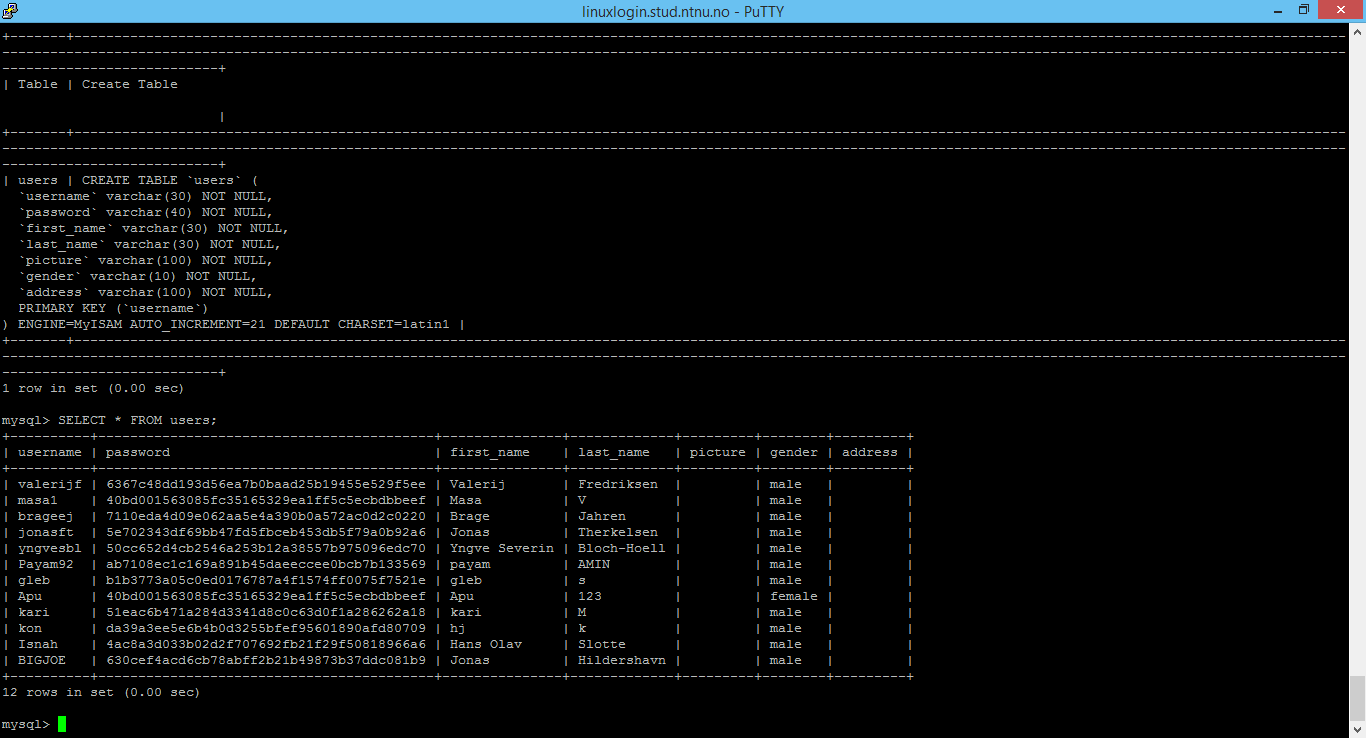
\includegraphics[width={\linewidth}]{Sprint2/img/Sprint2-testing.png}
\caption{ Testing of creating users was done at the end of the sprint, by using PuTTY and SQL checking that users were created correctly and if invalid users were found and caught. \label{overflow}}
\end{figure}

\section{Sprint Retrospective} 
\label{sec:S2Retrospective}

%TODO !!!!!!!!!!!!!!!!!!!!!!!!!!!!!!!!!!!!!!!!!!!!!!!!!!!!!!!!!!!!!!!!!!!!!!!!!!!!!!!!!!!!
%TODO !!!!!!!!!!TOTAL REWRITE ALERT !!!!!!!!!!!!!!!!!!!!!!!!!!!!!!!!!!!!!!!!!!!!!!!!!!!!!!
%TODO !!!!!!!!!!!!!!!!!!!!!!!!!!!!!!!!!!!!!!!!!!!!!!!!!!!!!!!!!!!!!!!!!!!!!!!!!!!!!!!!!!!!

\subsection{Start doing}
\label{subsec:S2RetrospectiveStart}
\begin{itemize}
\item Using the now set up Git, GitHub, IntelliJ technology for development of system and report.
\item Look into the use of YouTrack by Jetbrains for our agile development, to track progress of the project and sprint. 
\item Use the same naming conventions for development items to avoid ambiguity and inconsistency. All names in lowercase. 
\begin{itemize}
\item Back end PHP files: \\ db - PHP folder code that queries SQL.
\item img - Images resource folder. 
\item js - JavaScript files
\item styles - CSS folder for styling the page items. 
\end{itemize}
\item Set up new branches when starting to work on new functions of the page that are unrelated to the other branches. 
\item The Scrum Master needs to focus more on Scrum, sprints and work assignment.
\end{itemize}

\subsection{Continue doing}
\label{subsec:S2RetrospectiveContinue}
\begin{itemize}
\item Continue learning skills for the project.
\item Structurize the folders that have come out of structure. 
\item Use NTNU Home Area, MySQL server over SSH for running and testing code and testing database.
\end{itemize}

\subsection{Group Dynamics}
\label{subsec:S2RetrospectiveDynamics}

Although the number of work hours on average for each group member still did not match the goal of 20 hours, the team were getting closer. Comparing the first sprint work hours to the second, we could see an increase of 2\%.

\paragraph{} The members of the group are quite different and also work differently. When it comes to sprint work assignments, some members felt that the the tasks assigned were not specified well enough and because of this they had trouble starting their tasks. As a consequence, developing a more concrete sprint backlog with better estimations and task specifications were set as an important goal for the next sprint.

\paragraph{} So far the Scrum methodology were not been well implemented into the group's work. The group aims to improve on following the Scrum methodology points more accurately, rather than working as freely as done up until now. We plan to solve this problem by more clearly working by our role allocations.

\paragraph{} As earlier stated as a risk factor, the groups inexperience is also a challenge. As most members had no previous experience with web development, it was a challenge for several members to work effectively or start doing their tasks. Different members were trying different approaches to development, so to solve this issue we ensured that everyone was using the same development environments by the end of the sprint. 

\paragraph{} As the design, implementation and testing of Sprint 2 took place a couple of questions regarding user anonymity arose. The final product is aimed at end users being teenagers in the age range from ten to 25, and therefore there are pros and cons to how a user is displayed relative to other users. The team came up with three different ways to display users. 

\begin{description}
\item[Custom username: ] Teenagers can hide behind anonymous usernames. For the bullies, this makes it easier to post negatively or harass other users on the website, as it is difficult for other usernames to figure out who is behind a custom username. The only time full names are known with this solution is when users are joining the same events. 
\item[First name: ] This is a more neutral approach. It is easier to identify who users are, but difficult to know who is who for sure. Full name is still only available to the people joining the same events.
\item[Complete name: ] Everyone will be able to identify who a user is, and people already vulnerable to bullying and harassment might be at harm. Though this solution to the case would also make most users skeptical to post negatively because it would reflect badly on themselves. 
\end{description}


\subsection{Customer Feedback}
\label{subsec:S2RetrospectiveFeedback}
Upon seeing the latest changes to the product the customer was pleased with our work, and yet again impressed. As the customer does not have much experience with the technology being used and web development, the group's judgement and choices are usually sought and approved for the questions the team asks. Questions for this session was about general color changes and how to process the case of user anonymity on the page. Both parts came to a temporary agreement that custom usernames would be used for general display of usernames, and that the team would choose color preferences as they wished.
